% Options here are passed to the article class.
% Most common options: 10pt, 11pt, 12pt
\documentclass[10pt]{datasheet}

% Input encoding and typographical rules for English language
\usepackage[utf8]{inputenc}
\usepackage[english]{babel}
\usepackage[english]{isodate}

% tikz is used to draw images in this example, but you can
% also use \includegraphics{}.
\usepackage{graphicx}
\usepackage{float}
\usepackage{subcaption}

% These define global texts that are used in headers and titles.
\title{CH02: Parallelized Encoded Chest Hall Using Discs}
\author{JayRoi}
\tags{chest-halls, parallelized, decimal-encoding, hopperlocked, 10-chests, disc-encoding}
\date{25 December 2024}
\revision{Revision 1}
\begin{document}
\maketitle

\section{Features}
\begin{itemize}
\item{540 chests, 10 chests per slice.}
\item{25 block wide slices.}
\item{Fully parallelizable (10x hopperspeed for items, 1x hopperspeed for box insertion)}
\item{100\% hopperlocked with sectional unlocking}
\item{Self-repairable toggle states with Auto-Fix sequence}
\end{itemize}

\section{General Description}
The CH02 Parallelized Encoded Chest Hall Using Discs is a demonstrative prototype of a parallelized unloading logic inspired by Andrews54757's chest hall. However, the system is designed to be more compact and efficient by using discs to encode the chest locations instead of embedded redstone memory.

Single shulkerboxes and their codes can be custom ordered to specific unloading conditions as chosen by the player, though the intention is these orders would be externally automated. Orders can be programmed to unload a single box to a certain amount from the box, insert additional boxes, or only insert boxes. The hall can process up to 10 orders at a time, allowing for roughly 10x hopperspeed parallelization. 

\vfill\break

\begin{figure}[H]
    \centering
    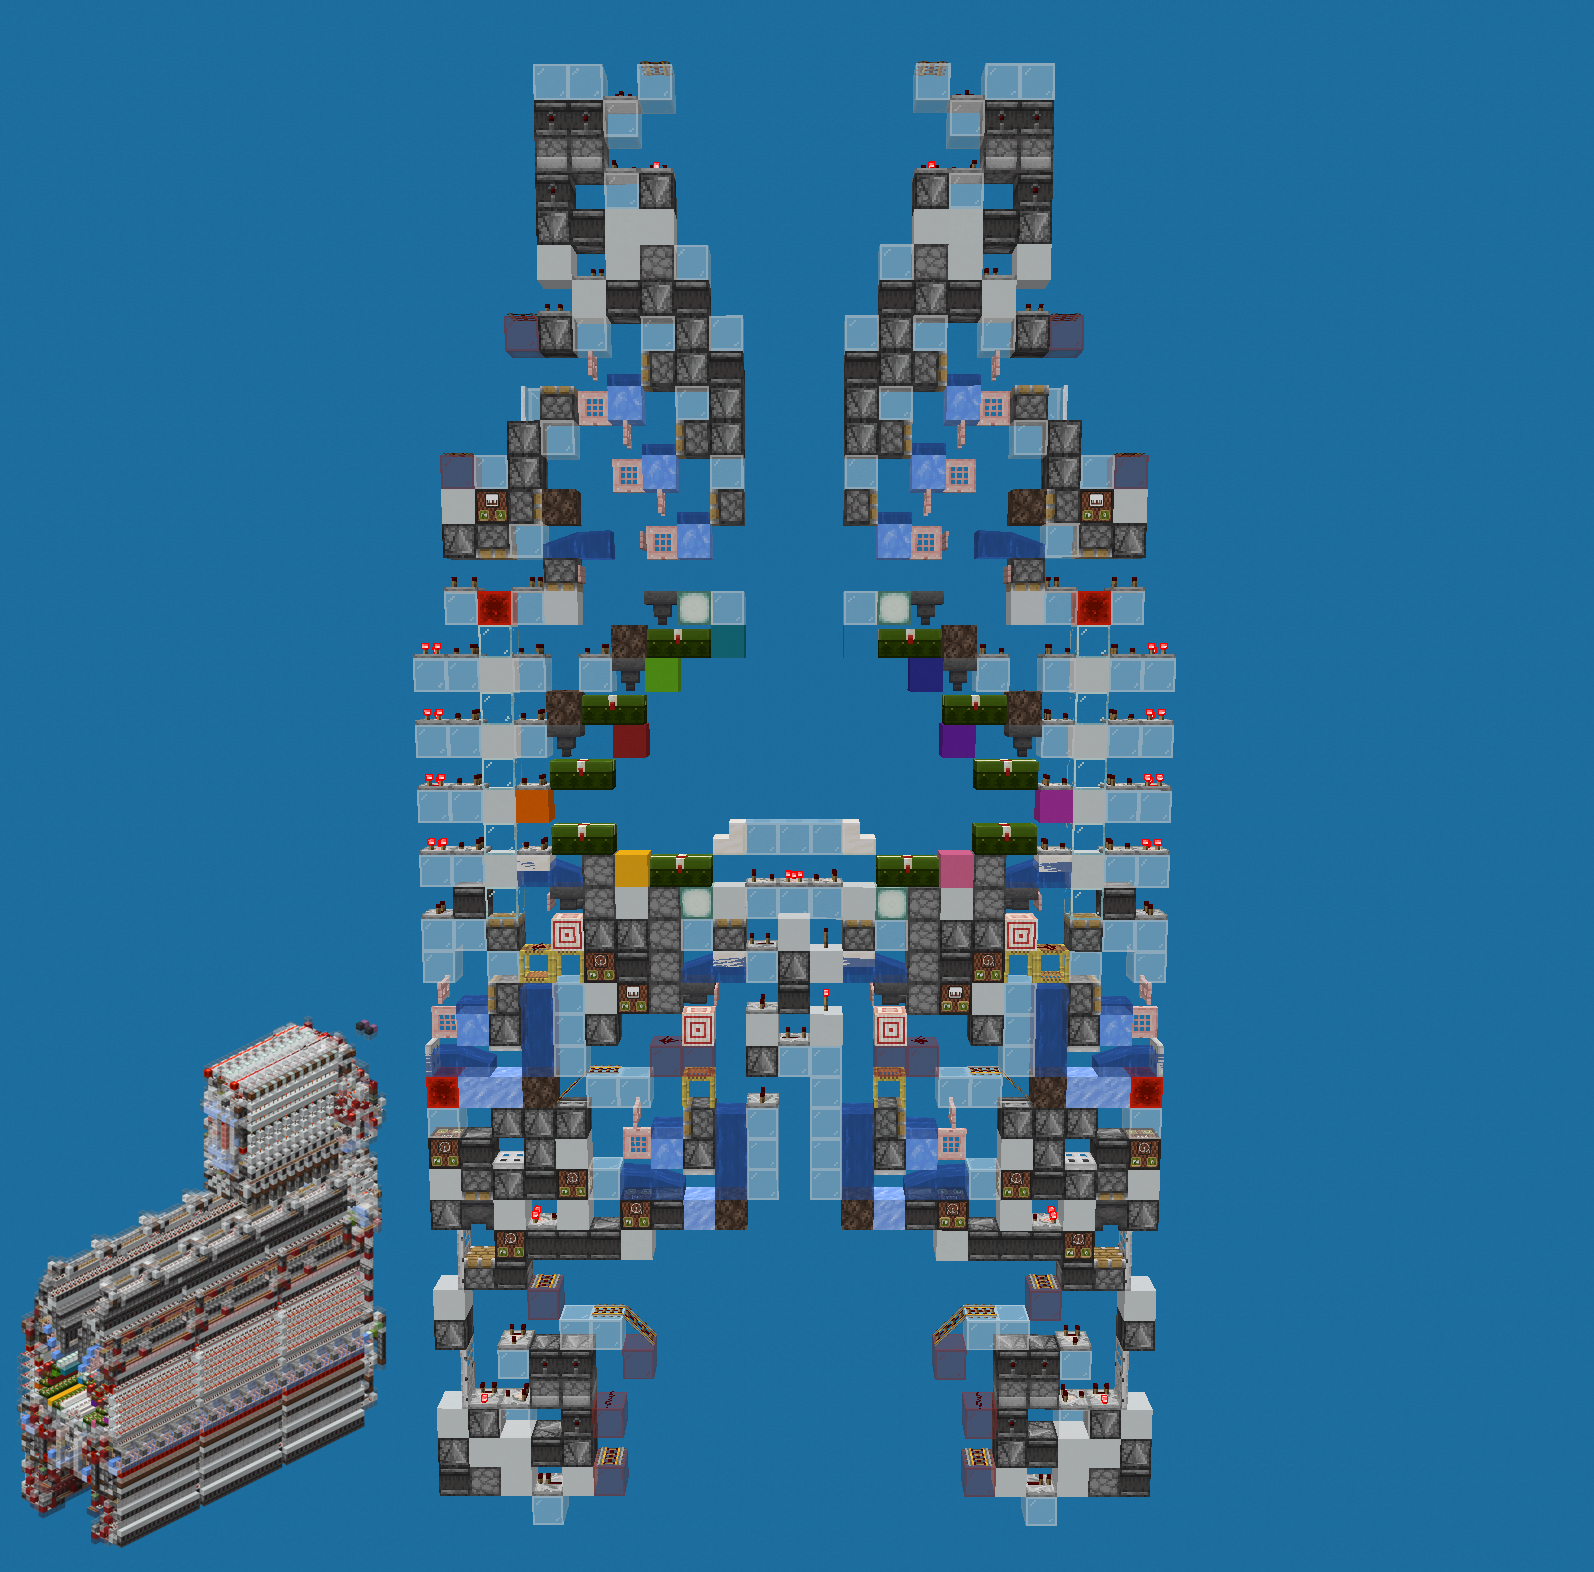
\includegraphics[width=0.48\textwidth]{pic.png}
    \caption{\centering Parallelized Encoded Chest Hall Using Discs}
\end{figure}

% For wide tables, a single column layout is better. It can be switched
% page-by-page.
\onecolumn

\section{Usage Instructions}
Procedure:
\begin{enumerate}
    \item Ensure the 8gt stabilizer is on, it is below the UI signified with a gold block.
    \item Insert the code box, the unloading box, and any additional boxes to be directly inserted.
    \item Make sure not to send any additional orders until the lamp indicates the system is ready.
    \item Next to the gold block/8gt stabilizer are noteblocks to depreciate the SS values determining the unloading amount. The clocks for these are not present as the system is incomplete.
    \item When the system is done, the chest-hall slices will not relock themselves as this feature is not completed, so click the locking button (on-top the doors) twice to turn the system off. Note: In practice, this noteblock can be clicked once every so often while the system is running to reduce lag.
\end{enumerate}

\section{Coding Instructions}

The first box of the order should be full with 3 or 4 music discs. The first 3 discs encode the address in the hall, and the fourth is used to determine how much of the box to unload (higher SS disc = more items). 
The second box will be unloaded (if chosen), and any additional boxes will be directly sent to the address.
To the right of the UI, there is a labeled lever to directly insert boxes of unstackable items, rather than unloading them. Note: The hall cannot unload unstackables at a separate rate than 16 or 64 stackables. 
Under this lever, there is a noteblock which will let you bypass unloading and directly insert the first box into the address.

\newpage

\section{Device Specifications}

\begin{table}[H]
    \caption{Device Specifications}
    \begin{tabularx}{\textwidth}{l | c c c | c | X}
        \thickhline
        \textbf{Parameter} & \textbf{Min.} & \textbf{Typ.} & \textbf{Max.} &
        \textbf{Unit} & \textbf{Conditions} \\
        \hline
        Throughput  & 1 & - & 10 & HS & Normal Usage \\
        \hline
        Hopper Count & & 597 & & Hoppers & \\
        \hline
        MC Version & 1.20 & 1.20.1 & - & MCV & Latest version at time of writing: 1.19.2\\
        \hline
        Dimensions & & 25 x 71 x 65 & & Blocks & \\
        \thickhline
\end{tabularx}
\end{table}

\section{Testing Data}

\begin{table}[H]
\caption{Executed Tests}
\begin{tabularx}{\textwidth}{l | X}
    \thickhline
    \textbf{Test} & \textbf{Result} \\
    \hline
    Item insertion & Items were successfully inserted in specific locations in parallel. \\
    \thickhline
\end{tabularx}
\end{table}

\section{Download Information}
\begin{table}[H]
    \caption{Download Information}
    \begin{tabularx}{\textwidth}{l | l | l | X}
        \thickhline
        \textbf{Identifier} & \textbf{MC} & \textbf{File} & \textbf{Description} \\
        \hline
        CH02 & 1.20.1 & \href{https://github.com/Soontech-Annals/Archive/blob/b56572c0d2b4f182d9e9d41449d8cb2963b923ae/Archive/chest-halls/CH02\%20Parallelized\%20Encoded\%20Chest\%20Hall\%20Using\%20Discs/CH02\_Parallelized\_Encoded\_Chest\_Hall\_Using\_Discs.litematic?raw=1}{CH02\_Parallelized\_Encoded\_Chest\_Hall\_Using\_Discs.litematic} & Schematic of device. \\
        \hline
        \thickhline
    \end{tabularx}
\end{table}

\section{Related Components}
\begin{table}[H]
    \caption{Related Components}
    \begin{tabularx}{\textwidth}{ l | l }
        \thickhline
        \textbf{Identifier} & \textbf{Description} \\
        \hline
        CH01 & Parallelized Encoded Chest Hall \\
        \hline
        DC02 & 10BPS 2 Digit Decimal Decoder \\
        \thickhline
    \end{tabularx}
\end{table}

\end{document}

